\section{Week 9 - Memory}

%\begin{itemize}
    %\item In the system, memory can only be allocated in sizes of an even multiple of four kilobytes. What are the possible reasons for that?
    %\item In your implementation, memory is maintained using a bitfield structure. What would the differences be if a linked list structure is used?
    %\item What are the advantages and disadvantages of using a linked list structure?
%\end{itemize}

\textbf{Memory allocation in multiples of four kilobytes}

Discretizing memory into contiguous blocks, is a way to create an abstraction from direct addresses to a block of memory. This makes memory management more efficient, since only free/allocated blocks must be evaluates instead of every address themselves. Large blocks means fewer blocks to evaluate and faster memory management, but too large blocks results in inefficient use of memory. There is therefore a compromise between speed and how well memory can be utilized.

Blocks of memory is used in memory management algorithms such as page tables and virtual memory, where the the table sizes depend on the block sizes. As memory can be needed in various quantities, no optimal choice of memory block sizes exists, as it depends on the programs running. Empirically 4 kB works efficiently and works as a good compromise between speed and memory usage.

When evaluating block sizes with respect to cache, it is useful to have block sizes which divides the cache size without remainder. Otherwise the remaining cache would never be used. The cache sizes are in general a power of two, meaning it is divisible by 4 kB $= 2^{12}$ bytes, as long as cache is larger than 4 kB.

\textbf{Bitfield vs Linked list structure}

For memory management, there are in general two ways to keep track of memory; bitfields (also known as bitmaps) and free lists, as stated in the book Modern Operating Systems section 3.2.3 \cite{tanembaum} and seen in figure \ref{fig:mapvslist}. Both strategies divide memory up into page frames/indivisible chunks and manage the frames themselves. For a bitfield, a table is stored with information regarding to whether each frame is free or used. Additional information (as seen in the labs), may be stored in the table, such as what processes owns the used frames and the first frame of the block of allocated set of contiguous frames. Allocating memory using a bitfield is achieved by finding the needed free contiguous entries in the table. With a bitfield once memory is freed next to already free memory, the border between them disappears automatically, creating one large section of free memory. This means that no further operations are performed to merge free sections of memory, as compared to the linked lists structure.

\begin{figure*}
    \centering
    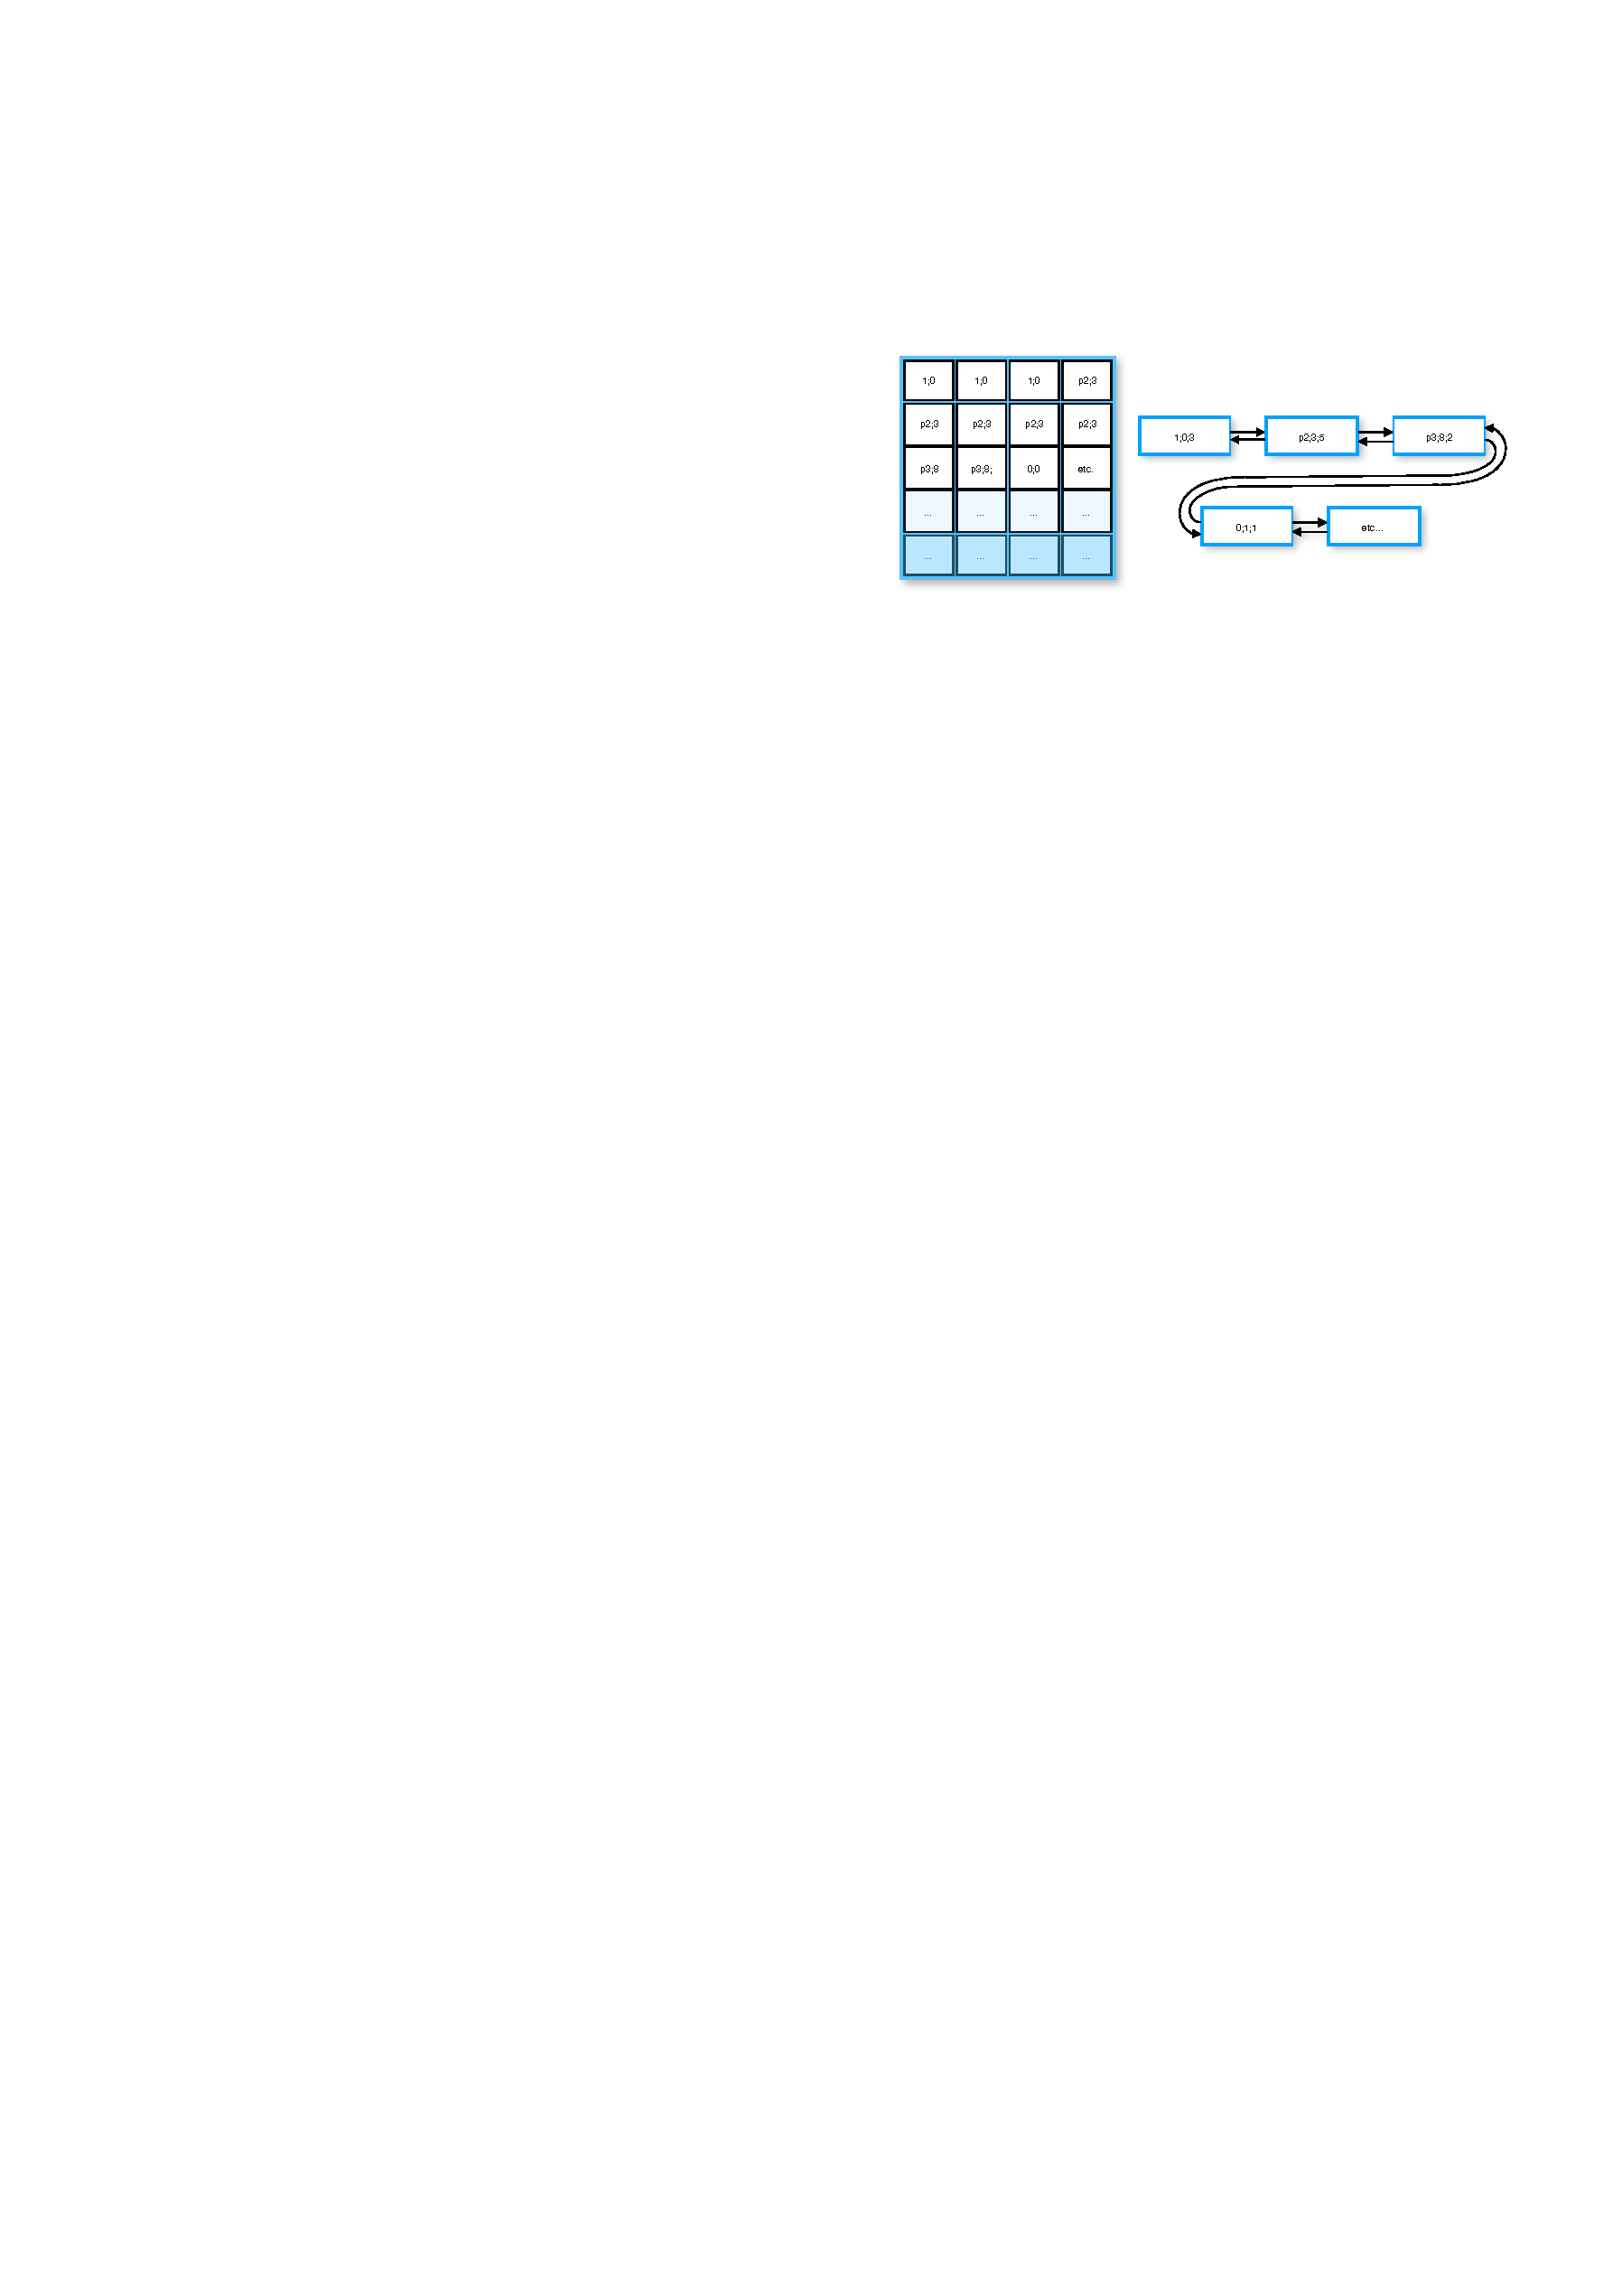
\includegraphics[width=0.7\textwidth]{fig/bitmatvslist.pdf}
    \caption{A bitmap/bitfield and a linked list representation of the same memory. The bitmap elements consist of a process pointer (where 1 is kernel and 0 is free) and a start index. The linked list elements consist of a process pointer, a start index and block size (together with pointers).}
    \label{fig:mapvslist}
\end{figure*}

When memory is managed with a linked list, each entry of the list contains four values; the process using the memory (if allocated) or a hole (if free), the starting index of the section, the size of the section and a pointer to the next element in the list. This way, when memory is allocated, the list is traversed and once an element corresponding to a hole of the correct size (most similar, first or largest depending on the allocation strategy, discussed further in the book \cite{tanembaum} section 3.2.3) is found, the memory is allocated. Finding memory slots may therefore be easy with a list, but once memory is freed, there is a risk of getting fragmented memory. When memory is freed, and the memory next to it is free also, they must be merged to one element in the list. For better performance, a double linked list may be preferred, to check the element before it in the list. Likewise when memory is allocated and a hole of larger size is found, it must be split into the allocated memory and a hole of remaining size.

Since the linked list dynamically creates elements at runtime, it must be possible to allocate memory for the elements themselves, meaning that special memory management for the list data structure must be available. Since the bitfield is of constant size, this problem does not occur, although the bitfield in general will use more memory, multiple entries in the table may hold the same information, as compared to the list.

\textbf{Lab implementation of page frames}

The kernel is set up with an array of page frames corresponding to the available memory for the system. The kernel itself uses a portion of these page frames, and these page frames are set as used and not deallocatable, meaning that no other process can accidentally or maliciously deallocate and overwrite kernel memory. The page management is implemented in the system calls \texttt{allocate} and \texttt{free}, which respectively allocates a set of contiguous free pages of a specified size, or frees an allocated memory block given the start page address from the block.

When allocating memory it is therefore necessary to first calculate the needed amount of pages to account for the requested amount of bytes, and find a spot of contiguous page frames in the page frame table. If such a spot in the page frame table is found, the members of the pages themselves are updated with respect to the start of the block and calling process, and an address to the allocated memory is returned. If no spot in the table is large enough \texttt{ERROR} is returned.

When freeing a memory block, we first want to be make sure that the complete block is allowed to be deallocated. The table is checked starting at the head of the block and continuing as long as the the page frames refer to the head of the block as the start of their block. If all page frames in the block are allowed to be freed, their owner and start index is reset, otherwise, if just a single page frame in the block is owned by another process or is not deallocatable, \texttt{ERROR} is returned and the memory is unchanged.